\documentclass[aspectratio=169]{beamer}
\usetheme{metropolis} % Use metropolis theme

\usepackage[ngerman]{babel}
\usepackage{amsmath}
\usepackage{amssymb}
\usepackage{mathtools}
\usepackage{graphicx}
\usepackage{raleway}

\title{Rolling-bouncing ball - Dynamik eines Balles}
\author{Helene Rößler, Norbert Hammer}
\date{}


\begin{document}
\maketitle

\section{Bewegungsgleichungen}

\begin{frame}{Massenpunkt auf einer Kurve}
\begin{itemize}
    \item Ball als Massepunkt modelliert
    \item Bewegung auf Kurve gegeben durch $G(q)=0$
    \item Lösungskurve $q(t)$
    \item Das Variationsprinzip
    \begin{equation*}
        0 = \delta \int_0^T L(q, \dot{q}) \boldsymbol{ + \lambda G(q)} \ dt
    \end{equation*}
    \item führt zu
        \begin{align*}
            m \ddot{q} &= F + \lambda \nabla G(q)\\
            0 &= G(q).
        \end{align*}
\end{itemize}
\end{frame}

\begin{frame}{Massenpunkt auf einer Kurve}
\begin{itemize}
    \item In zweiten Ableitungen ausgedrückt:
        \begin{equation*}
        \underbrace{
        \begin{pmatrix}
          m & 0 & 0 \\
          0 & m & 0 \\
          0 & 0 & 0
        \end{pmatrix}}_{\eqcolon M ~ \text{(Massenmatrix)}}
        \begin{pmatrix} \ddot{q} \\ \ddot{\lambda} \end{pmatrix} =
        \begin{pmatrix}
          F + \lambda \nabla G(q)\\
          G(q)
        \end{pmatrix}
        \end{equation*}
\end{itemize}
\end{frame}

\begin{frame}{Massenpunkt im freien Fall}
\begin{itemize}
    \item ohne Nebenbedingung $G(q)=0$
    \item Das Obige wird zu
        \begin{equation*}
            F = \begin{pmatrix}
            m & 0 \\
            0 & m
            \end{pmatrix} \ddot{q}.
        \end{equation*}
\end{itemize}
\end{frame}

\section{Krümmung einer impliziten Kurve}

\begin{frame}{Krümmung einer Kurve}
\begin{itemize}[<+->]
    \item Sei $\varphi (t)$ Parameterdarstellung einer Kurve.
    \item<.-> Krümmung ist gegeben durch
        \begin{equation*}
        \kappa = \frac{\varphi_1'(t) \varphi_2''(t) - \varphi_2'(t) \varphi_1''(t)}{\| \varphi '(t) \|^3}.
        \end{equation*}
    \item Problem: Wir kennen $\varphi$ nicht!
    \item<.-> Beachten Sie: $\kappa$ nicht von Wert von $\varphi$ abhängig,
        nur von Ableitungen
    \item<.-> Lösung des Problems: Hauptsatz über implizite Funktionen
\end{itemize}
\end{frame}

\begin{frame}{Krümmung einer Kurve}
\begin{itemize}[<+->]
    \item Hauptsatz liefert erste (und damit auch zweite) Ableitung von Funktion,
        die mit Kurve übereinstimmt
    \item Problem: Kurve muss lokal als Funktion darstellbar sein
    \item Lösung:

    \begin{tabular}[t]{l c}
    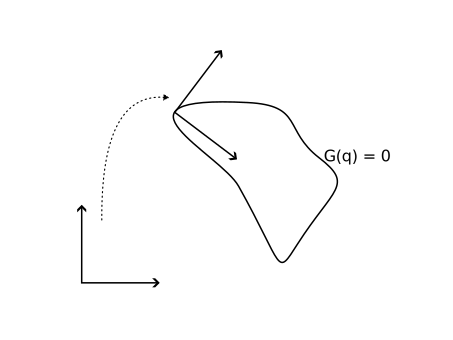
\includegraphics[scale=0.7]{./trafo.png} &
    {$\!\begin{aligned} % http://tex.stackexchange.com/q/98482/16595
        \nu &= \frac{ \nabla G(x_0) }{ \| \nabla G(x_0) \| } \\
        \tau &= (-\nu_2, \nu_1)
        \end{aligned}$}
    \end{tabular}
\end{itemize}
\end{frame}

\begin{frame}{Krümmung einer Kurve}
\begin{itemize}
    \item Krümmung des Graphen der Funktion $f(t)$:
        \begin{equation*}
        \kappa = \frac{f''(t)}{(1 + f'(t)^2)^{3/2}}.
        \end{equation*}
\end{itemize}
\end{frame}

\begin{frame}{Zentrifugalkraft auf einer Kurve}
\begin{itemize}
    \item Massepunkt mit Position $q$, Masse $m$
    \item offizielle Vektorform:
        $$
        \hat{F}_c = m ~ \omega \times (q \times \omega).
        $$
    \item für eine
\end{itemize}
\end{frame}

\end{document}
